\chapter{Phase 1}
\label{ch:phase1}

Phase~1 built and tested the vision core of the system on a laptop with an
NVIDIA RTX~4060 GPU: plate detection, weather restoration, plate reading, and
the tracking and voting that turn per-frame readings into confirmed plates.
This chapter describes the implementation and the results in the order in
which the pipeline processes a frame. The work was done in steps in which each
result decided the next one; where an approach did not help, the evidence is
reported as well, because those negative results shaped the final design.

% ---------------------------------------------------------------------
\section{Plate Detection with YOLOv11}
\label{sec:yolo}

\subsection{Implementation}

A YOLOv11n detector with one class (licence plate) was trained with the
Ultralytics framework. A first model trained on a small set of labelled images
(51 epochs, stopped early at epoch 31) reached mAP@50 of 0.931 and was used
to build the first versions of the pipeline. The final detector was trained for
100 epochs on a set of more than 15\,000 annotated licence-plate images, and is
run at an input size of 1280 pixels with a confidence threshold of 0.25 so that
small plates in 1080p and 4K frames are not lost.

\subsection{Results and Discussion}

Training and validation losses fell steadily and the validation metrics levelled
off (Figure~\ref{fig:yolocurves}). The final model reached a precision of
98.5\,\%, a recall of 99.0\,\%, a mAP@50 of 99.2\,\% and a mAP@50--95 of
85.6\,\% on the validation set (Table~\ref{tab:yolo}). The normalised confusion
matrix (Figure~\ref{fig:yoloconf}) shows that 99\,\% of plates were found and
about 1\,\% of background regions were wrongly detected. Predictions on
validation images have a confidence of about 0.9 on every plate
(Figure~\ref{fig:yolopred}).

\begin{figure}[t]
\centering
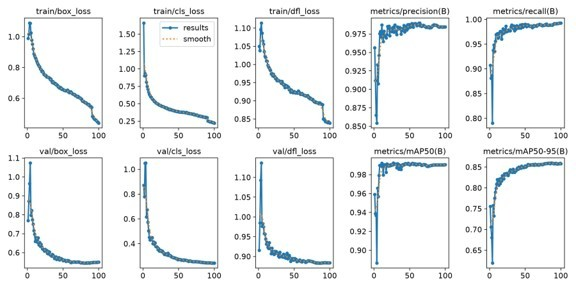
\includegraphics[width=0.92\textwidth]{yolo_curves.png}
\caption{Training and validation curves of the YOLOv11n plate detector.}
\label{fig:yolocurves}
\end{figure}

\begin{table}[t]
\centering
\caption{Plate detector results on the validation set.}
\label{tab:yolo}
\begin{tabular}{@{}lc@{}}
\toprule
\textbf{Metric} & \textbf{Validation result}\\
\midrule
Precision & 98.5\,\%\\
Recall & 99.0\,\%\\
mAP@50 & 99.2\,\%\\
mAP@50--95 & 85.6\,\%\\
\bottomrule
\end{tabular}
\end{table}

\begin{figure}[t]
\centering
\begin{subfigure}[b]{0.46\textwidth}
  \centering
  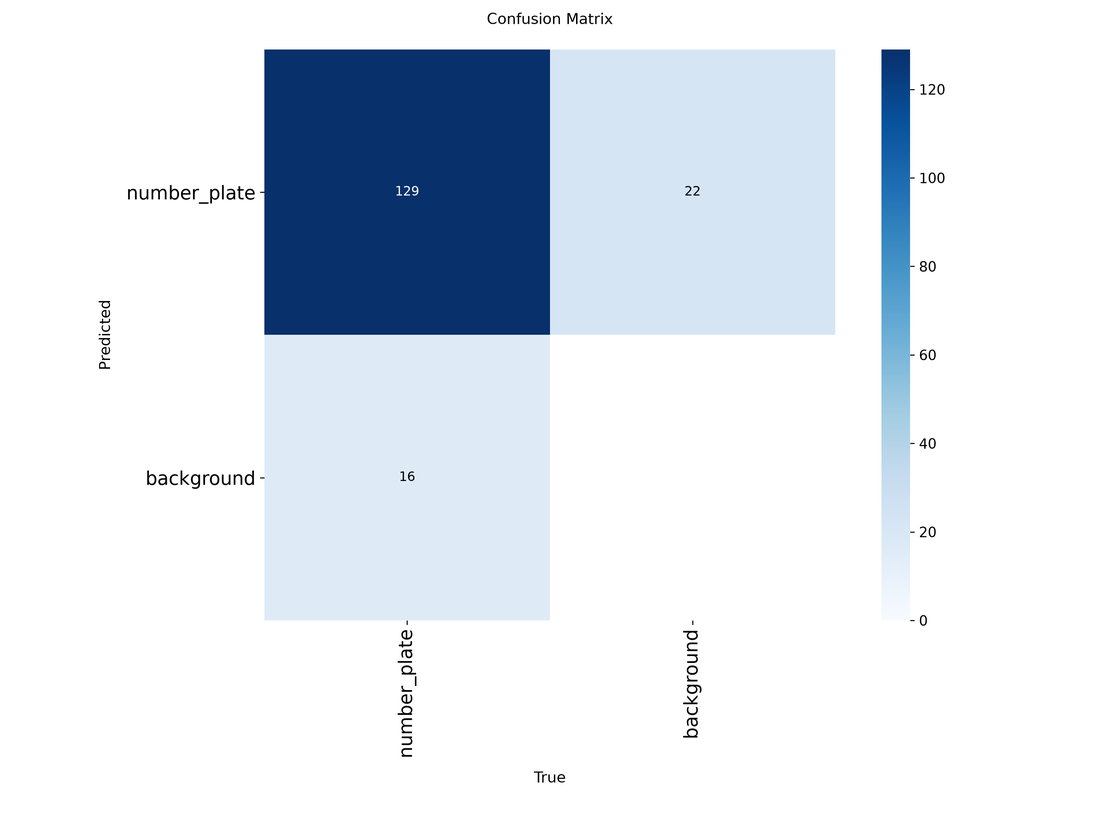
\includegraphics[width=\textwidth]{yolo_confusion.png}
  \caption{Normalised confusion matrix.}
  \label{fig:yoloconf}
\end{subfigure}\hfill
\begin{subfigure}[b]{0.46\textwidth}
  \centering
  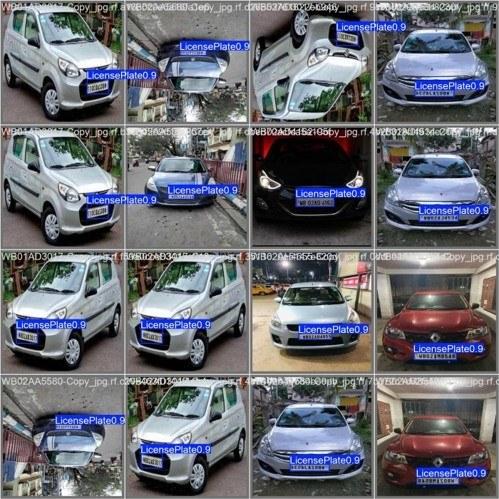
\includegraphics[width=\textwidth]{yolo_predictions.jpg}
  \caption{Predictions on validation images.}
  \label{fig:yolopred}
\end{subfigure}
\caption{Detector evaluation.}
\label{fig:yolo}
\end{figure}

On video the detector is the limit for the smallest plates. The plates of
two-wheelers and autos are only about 22--39 pixels wide; they are found at a
confidence of 0.1 and a minimum size of $14\times8$ pixels, but the reader
cannot read them reliably. A detector fine-tuned at 1280 pixels on 65
hand-corrected traffic frames together with the earlier sets raised recall on
23 hand-labelled frames from 74\,\% to 87\,\%, but it was \emph{not} adopted:
on the benchmark video the reader got fewer plates right with its boxes
(15 against 20 of 27), so the original detector remains in use. On the 60
Ponmudi photos of Section~\ref{sec:ponmudi}, lower thresholds, a larger input
size and tiled detection found 44 additional boxes, but only three of them
read as valid plates, so the baseline detector was kept there too.

% ---------------------------------------------------------------------
\section{Weather Restoration}
\label{sec:restoration}

\subsection{First comparison: DCP, a transformer network and CLAHE}
\label{sec:first}

Three restoration methods were compared on the 1\,001-image Foggy-Hazy plate
set and on a real foggy road photograph. Every result is the actual EasyOCR
reading of the output, not a visual impression.

\paragraph{Dark Channel Prior.} On mild haze DCP helped: the confidence of the
plate reading rose from 0.227 to 0.336 (about 48\,\% relative) and the text came
out cleaner (Figure~\ref{fig:dcp}a). On dense, nearly uniform fog it failed.
With gentle settings the output was identical to the input (mean confidence
0.326 for both), and with stronger settings ($\omega=0.6$, $t_{\min}=0.10$) the
whole frame collapsed to white (Figure~\ref{fig:dcp}b).

\begin{figure}[t]
\centering
\begin{subfigure}[b]{0.52\textwidth}
  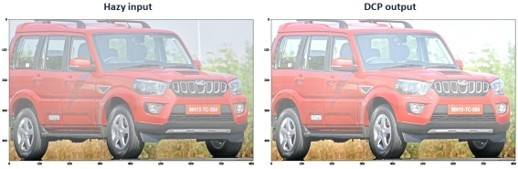
\includegraphics[width=\textwidth]{dcp_mild.png}
  \caption{Mild haze: ``MH15 TC 554'' (0.227) became ``Mh1s-TC 554'' (0.336).}
\end{subfigure}\hfill
\begin{subfigure}[b]{0.44\textwidth}
  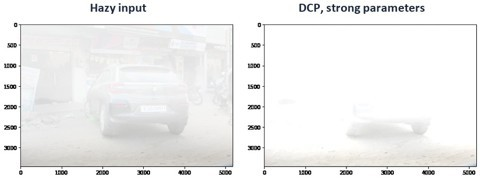
\includegraphics[width=\textwidth]{dcp_dense.png}
  \caption{Dense haze with strong settings.}
\end{subfigure}
\caption{DCP on mild and dense haze (hazy input left, output right).}
\label{fig:dcp}
\end{figure}

\paragraph{Transformer U-Net.} A transformer dehazing network
(window-attention blocks in the bottleneck) trained on synthetic hazy and clear
pairs made from 250 clear plate crops reached a PSNR of 21.76~dB, raised to
22.68~dB with a lower learning rate, a larger model and filtering of blurry
source images (250 to 242 crops). It gave the cleanest-looking reconstruction
of the car, but it smoothed away the fine edges that OCR needs: its mean OCR
confidence was 0.104 against 0.326 for the hazy input, and its readings were
fragments such as ``Wui'' and ``Www''. Higher PSNR did not give better OCR.

\paragraph{CLAHE.} CLAHE was the only method that recovered a plate where the
input and DCP gave nothing: ``KL 55R 2473'' at confidence 0.774
(Figure~\ref{fig:clahe}b). It was not consistent: on the mild-haze photograph
it made the reading worse (0.227 to 0.097), and on the real foggy road
photograph the scene contrast improved but the plate, only about 33 pixels tall
and optically blurred, stayed unreadable. CLAHE is also the fastest method,
about 1.3~ms per image against 17~ms for DCP.

\begin{figure}[t]
\centering
\begin{subfigure}[b]{0.6\textwidth}
  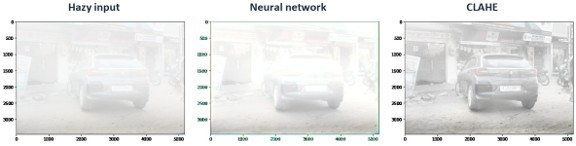
\includegraphics[width=\textwidth]{neural_vs_clahe.png}
  \caption{Hazy input, neural network output and CLAHE output.}
\end{subfigure}\hfill
\begin{subfigure}[b]{0.37\textwidth}
  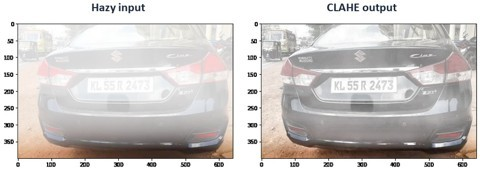
\includegraphics[width=\textwidth]{clahe_recovered.png}
  \caption{CLAHE recovered ``KL 55R 2473'' (0.774).}
\end{subfigure}
\caption{The dense-haze frame under the neural network and CLAHE, and the plate
that CLAHE recovered.}
\label{fig:clahe}
\end{figure}

\begin{table}[t]
\centering
\caption{First comparison of restoration methods (OCR confidence; ``--'' means
not tested).}
\label{tab:first}
\small
\begin{tabular}{@{}lcccc@{}}
\toprule
\textbf{Example} & \textbf{Input} & \textbf{DCP} & \textbf{Neural} & \textbf{CLAHE}\\
\midrule
Mild haze (plate confidence) & 0.227 & 0.336 & -- & 0.097\\
Heavy uniform haze (mean, no plate found) & 0.326 & 0.326 & 0.104 & 0.313\\
Moderate haze (plate confidence) & not found & not found & -- & 0.774\\
Heavy haze, other scene & not found & not found & -- & not found\\
Real foggy road photo & not found & -- & -- & not found\\
\bottomrule
\end{tabular}
\end{table}

Over 20 randomly sampled hazy images the mean OCR confidence was 0.309 (hazy),
0.326 (DCP, gentle settings), 0.114 (neural network) and 0.320 (CLAHE). No
method was reliably better than the others, and where the limit is the
resolution or optical blur of the source no method recovers a reading. CLAHE
was therefore chosen as the first restoration route because it is the fastest
and never fails badly (Table~\ref{tab:first}).

\subsection{UVMNet for fog removal}
\label{sec:uvm}

\paragraph{Why a second network.} The transformer network of the previous
section was trained only on synthetic pairs made from plate crops, and it
blurred plate text. A model trained on whole road scenes with real depth-dependent
fog was needed. UVM-Net~\cite{zheng2024uvmnet} combines a U-shaped
encoder--decoder with Mamba state-space blocks~\cite{gu2023mamba}. Our
implementation has 116.2 million parameters, predicts a residual that is added
to the input, uses batch normalisation, and runs with the real \code{mamba-ssm}
CUDA kernel under WSL2. Full-resolution photographs are processed in
overlapping tiles (tile size 1536, overlap 128) with feathered blending to avoid
seams, and a guided-filter step refines the output.

\paragraph{Training in stages.} The network was trained in stages, each answering
a problem found in the previous one (Table~\ref{tab:uvmstages}).

\begin{table}[t]
\centering
\caption{Training stages of UVMNet.}
\label{tab:uvmstages}
\small
\begin{tabularx}{\textwidth}{@{}p{2.1cm}X p{3.0cm}@{}}
\toprule
\textbf{Stage} & \textbf{Data and method} & \textbf{Result}\\
\midrule
A. Traffic haze & 8\,925 foggy/clear pairs (Foggy Cityscapes, 200 validation pairs), $384\times384$ crops with flips, mixed precision, 50 epochs & Validation PSNR 22.95 to 32.96~dB (epoch 42)\\
B. Plate fine-tune & 250 clear plate crops, 1\,968 hazy variants; combined loss (Charbonnier + gradient + residual regularisation); physically exact haze-density augmentation & Brightness retention on Foggy Driving 46\,\% to 70\,\%\\
C. Multi-dataset & RESIDE-OTS (15\,198 files), Foggy-Hazy plates (1\,001 real pairs), NH-HAZE (53 real pairs, oversampled); fp32 validation; feathered tiles & Best PSNR 27.30~dB (epoch 38); 9 of 10 real test photos clean\\
D. Variants tried & Low-light augmentation; CLAHE-preprocessed input & 26.33~dB with skipped batches; 19.7~dB; both dropped\\
\bottomrule
\end{tabularx}
\end{table}

Stage~A reached 32.96~dB on its own domain with no overfitting, but on photographs
of our own it produced a green colour cast and kept only about 46\,\% of the
ground-truth brightness, while domain-matched validation images were clean
(brightness ratio 0.98, 28.08~dB on 100 images); the cause was the gap between
training and test domains, not a code error. Stage~B protected brightness and
detail with the combined loss and the haze-density augmentation
\[
  I_{\text{new}} = J + \alpha\,(I - J),
\]
which is the exact result of sampling a different transmission in
Equation~\eqref{eq:fog} and was used to vary fog thickness. Stage~C added
public sets with real or large-scale fog. Validation had turned to NaN from
epoch 10 because of an fp16 overflow in an unscaled validation pass; validating
in fp32 and skipping non-finite batches fixed it. The remaining failure was a
dusk-time dense-fog highway photograph with an almost featureless plate area,
which neither low-light augmentation nor CLAHE preprocessing could fix.

\paragraph{Effect on reading.} On the 21 held-out Foggy-Hazy scenes the reader
read 40.5\,\% of plates exactly from raw hazy crops and 36.3\,\% after
dehazing, because the reader had only seen raw crops at that time. On 250
hazy Rajasthan plate photographs read with the later reader, the final
(format-corrected) readings were right on 205 of 248 restored images against
195 of 248 on the hazy originals, so restoration did help once the reader was
trained on a broader set of plates.

\subsection{Real fog at Ponmudi}
\label{sec:ponmudi}

Synthetic haze does not behave like mountain fog. To test the system on the
real thing, 60 photographs of parked and moving vehicles in fog were taken at
Ponmudi, a hill station in Kerala, and the 85 plates that are legible to a human
were read by eye and verified. The test is hard: a plate is on the order of
30--60 pixels wide, blurred by fog and grain, and the label noise of the set is
about $\pm3$ plates. The installed reader and dehazer were left unchanged while
the study ran.

\paragraph{Models trained for real fog.} Several UVMNet variants were fine-tuned
for this domain: a model fine-tuned on Ponmudi-style fog, one trained through the
guided filter (``filter-trained''), a ``GoPro hybrid'' trained with fog synthesised
from clear GoPro frames followed by a tint fix for the colour cast, and a
mixed model trained on aligned pairs (NH-HAZE, synthetic Ponmudi fog, GoPro-clear
synthetic fog) with additional losses that match the statistics of real fog
photographs (haze, saturation, grain) and exponential-moving-average weights,
mixed precision and batch-norm repair, with a preview image and PSNR after every
epoch. A longer run of the same mixed recipe was also tried.

\paragraph{Physics-guided dehazing.} Even a good network sometimes leaves ghost
trees at tile seams or changes colours. The physics-guided procedure uses the
network only to \emph{measure} the fog and removes it from the real photograph
with Equation~\eqref{eq:fog} (Figure~\ref{fig:physics}). In outline:
\begin{enumerate}
  \item The network output $J'$ is computed. Taking $A$ from the observed
        image, the transmission at each pixel is the least-squares solution over
        the colour channels of $I-A = t\,(J'-A)$, filled where the estimate is
        unreliable using a confidence weight and smoothed with a guided
        filter.
  \item The atmospheric light $A$ is taken from the brightest 0.1\,\% of the
        dark channel and clipped to a plausible range (0.55--0.97).
  \item The real photograph is dehazed by inverting the scattering law with a
        strength exponent $\gamma$ on the transmission ($\gamma>1$ removes
        more fog), a floor on $t$, and a cap of 1.5 on the detail gain.
  \item An exposure match brings the mean brightness to a fixed target so that
        removing the veil does not darken the picture.
\end{enumerate}
For video the veil colour and $\gamma$ are smoothed over time with exponential
moving averages (weights 0.2 and 0.15) so that the picture does not flicker.
The cleanest source for the measurement was a 50/50 blend of the GoPro hybrid
and the new mixed model; single tiled sources left seams and ghosts.

\begin{figure}[t]
\centering
\begin{tikzpicture}[node distance=6mm and 6mm]
  \node[blk] (img) {Foggy\\photo $I$};
  \node[blk,right=of img] (net) {UVMNet\\(measure only)};
  \node[blk,right=of net] (t) {Estimate $t$\\(least squares\\+ guided filter)};
  \node[blk,below=8mm of t] (A) {Estimate $A$\\(dark channel)};
  \node[grn,left=of A] (inv) {Invert\\$J=(I-A)/t^{\gamma}+A$};
  \node[grn,left=of inv] (exp) {Exposure\\match};
  \draw[arr] (img) -- (net);
  \draw[arr] (net) -- (t);
  \draw[arr] (img.south) -- ++(0,-4mm) -| (inv.north);
  \draw[arr] (t) -- (A);
  \draw[arr] (A) -- (inv);
  \draw[arr] (inv) -- (exp);
  \node[blk,below=8mm of exp] (outn) {Dehazed\\output $J$};
  \draw[arr] (exp) -- (outn);
\end{tikzpicture}
\caption{Physics-guided dehazing: the network supplies only the estimate of the
fog thickness $t$ and the veil $A$; the fog is removed from the real photograph
by inverting the scattering law.}
\label{fig:physics}
\end{figure}

\paragraph{Depth-aware synthetic fog.} Real fog thickens with distance, so a
second family of training data was synthesised from clear photographs with an
estimated depth map. Depth Anything~V2 (small)~\cite{yang2024depthanythingv2}
estimates relative depth, the optical thickness along the line of sight is
sampled log-uniformly between 0.6 and 4.5 for the far field and scaled by 0.22
for the near field, and the veil brightness is drawn between 0.58 and 0.90 and
calibrated against real photographs. A UVMNet trained on these pairs
(``depth-fog'') gained about 4~dB on its own held-out depth-fog test, but gave no
gain on the 60 real photographs.
\label{sec:depthfog}

\paragraph{Results.} The comparison used the exact number of the 85 plates read
by the reader after each restoration, together with objective haze and grain
measures of the pictures (Table~\ref{tab:ponmudi} and
Figure~\ref{fig:ponmudiread}). Three findings stand out.
\begin{enumerate}
  \item The best-looking pictures come from the physics-guided procedure with
        strong settings and exposure matching on the blended source; its haze
        measure is 0.261 with a grain level of 0.020, and the filter-trained
        UVMNet gives the lowest haze (0.207, against 0.536 for the raw UVMNet
        output), but looks over-smoothed.
  \item The number of plates read does not follow the look. Every dehazer
        raised the reading of the \emph{installed} reader from 40 to 44--49 of
        85, but a reader trained for weather read 47--51 on the \emph{untouched}
        photographs, and no dehazer pushed any reader beyond about 52. The
        depth-fog network, the longer mixed run and a plate-aware training loss
        (a frozen reader's loss fed through region-of-interest pooling, which
        raised held-out hazy plates from 34 to 39--40 of 53) all stayed inside
        the $\pm3$ noise on the Ponmudi set.
  \item Applying the guided filter to UVMNet output is needed (raw network
        output reads worse), but applying it to the output of the newest
        model hurt reading (39). Flipping and multi-scale averaging gave no
        gain and cost two to five times the time.
\end{enumerate}
The limit is therefore the information in the photographs, not the dehazer: a
plate that fog and grain have blurred cannot be recovered from a single frame.

\begin{table}[t]
\centering
\caption{Restoration choices on the 60 Ponmudi photographs (85 plates). Exact
plates are for the stated reader; the noise of the set is about $\pm3$.}
\label{tab:ponmudi}
\small
\begin{tabularx}{\textwidth}{@{}Xcc@{}}
\toprule
\textbf{Input to the reader} & \textbf{Reader} & \textbf{Exact (of 85)}\\
\midrule
Untouched photograph & installed & 40\\
UVMNet variants + guided filter & installed & 44--49\\
Physics-guided, strong + exposure (blend source) & installed & 49\\
Depth-fog network & installed & 46 (mean)\\
Untouched, ``select'' view & weather-trained & 47--51\\
Plate-aware dehazers (four variants) & installed & 44--52\\
\bottomrule
\end{tabularx}
\end{table}

\begin{figure}[t]
\centering
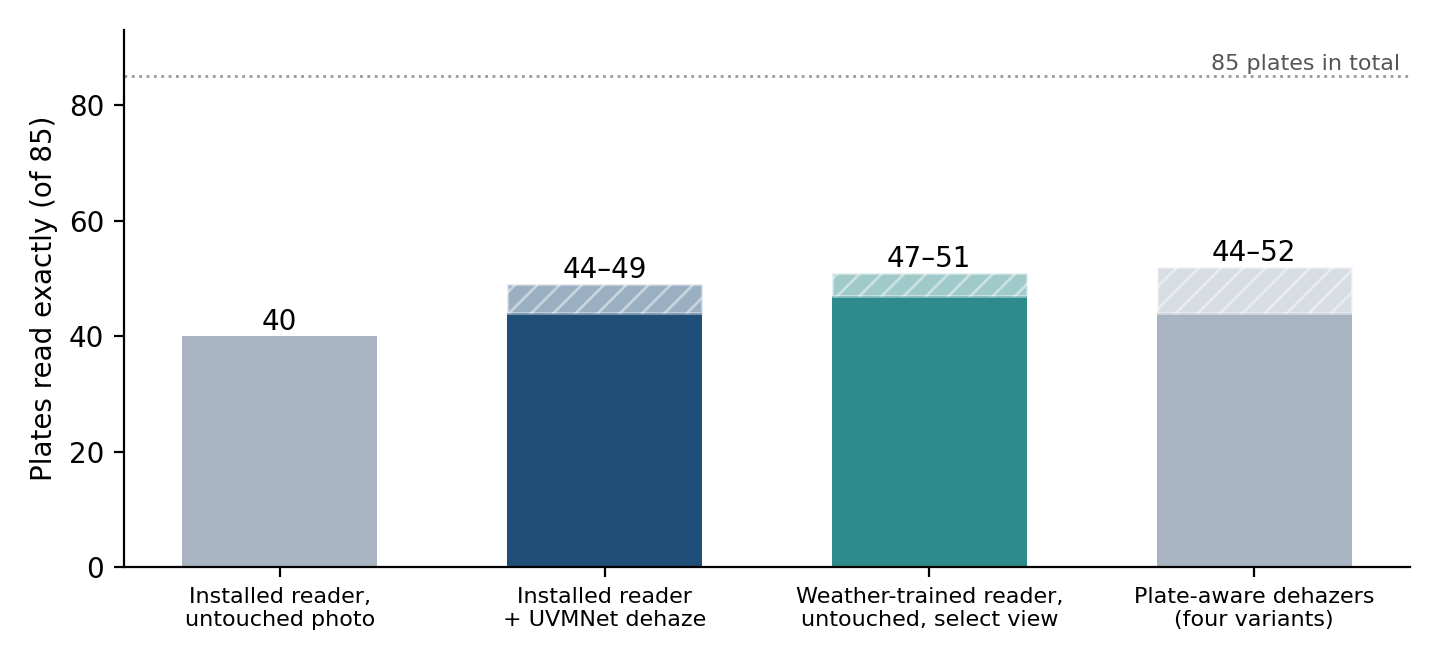
\includegraphics[width=0.8\textwidth]{ponmudi_reading.png}
\caption{Plates read exactly (of 85) for the main ways of preparing a Ponmudi
photograph (the hatched part is the range over the variants tried); all
dehazers lie in the same band as the weather-trained reader on the untouched
photograph.}
\label{fig:ponmudiread}
\end{figure}

Figure~\ref{fig:ponmudicmp} shows the original photograph, the GoPro-hybrid
model with tint fix, and the physics-guided result side by side for several
scenes. The restored pictures show the vehicles with natural colour and much
less veil, which is useful for operators watching a feed, even though the plate
reading is limited by the source.

\begin{figure}[p]
\centering
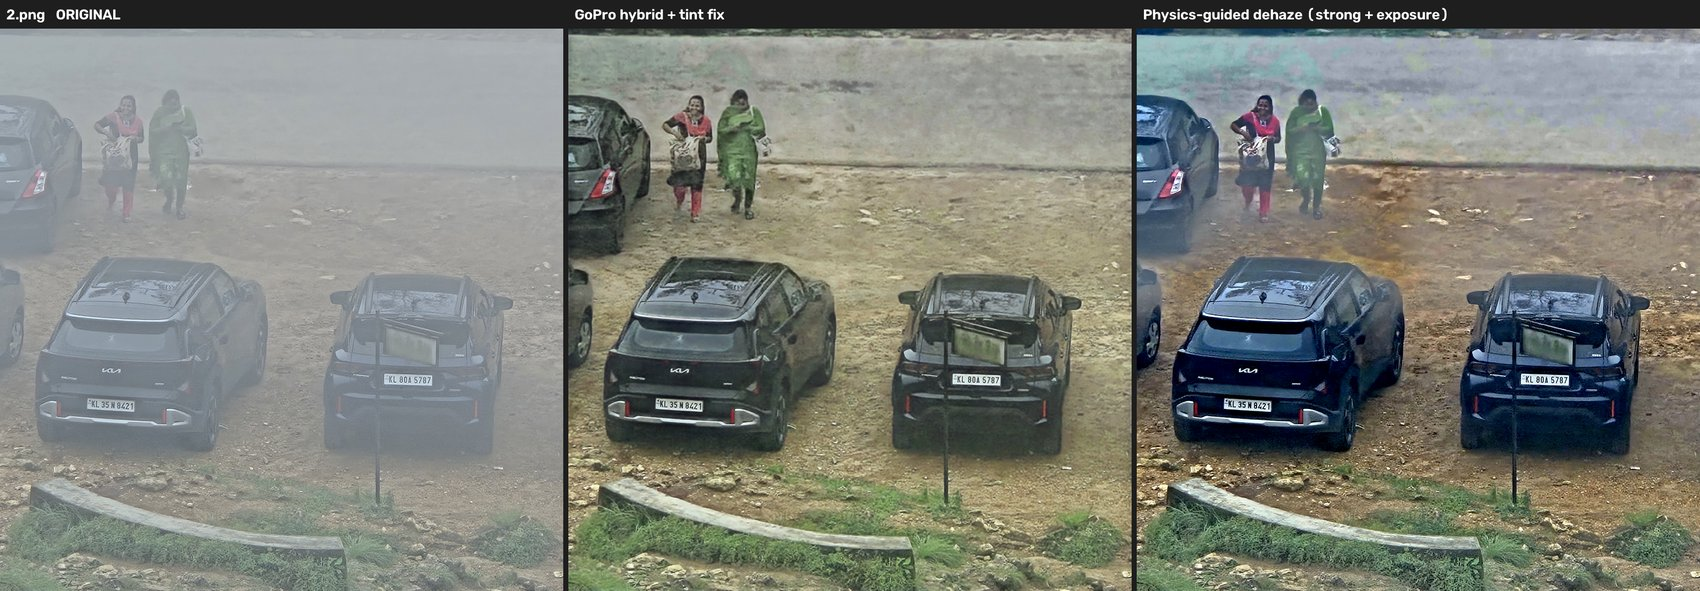
\includegraphics[width=\textwidth]{ponmudi_cmp_parking.jpg}\\[4pt]
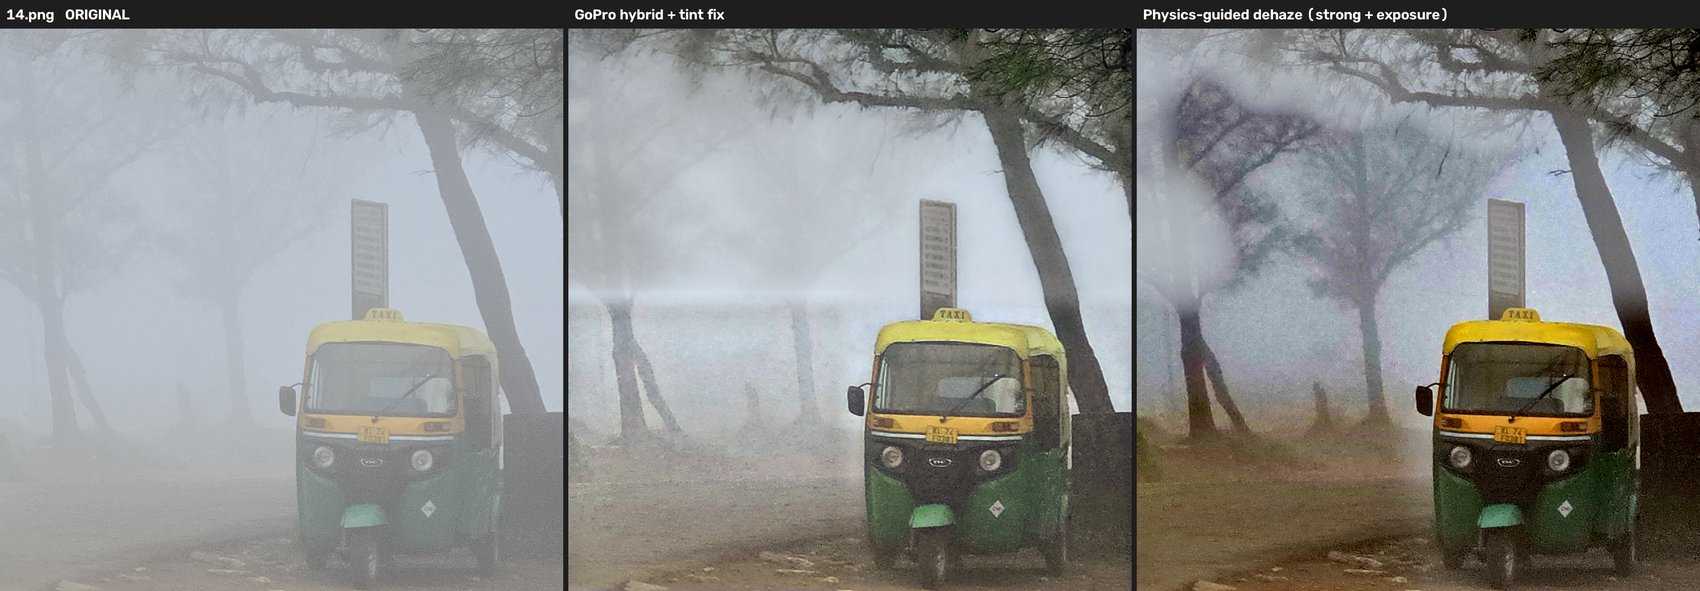
\includegraphics[width=\textwidth]{ponmudi_cmp_rickshaw.jpg}\\[4pt]
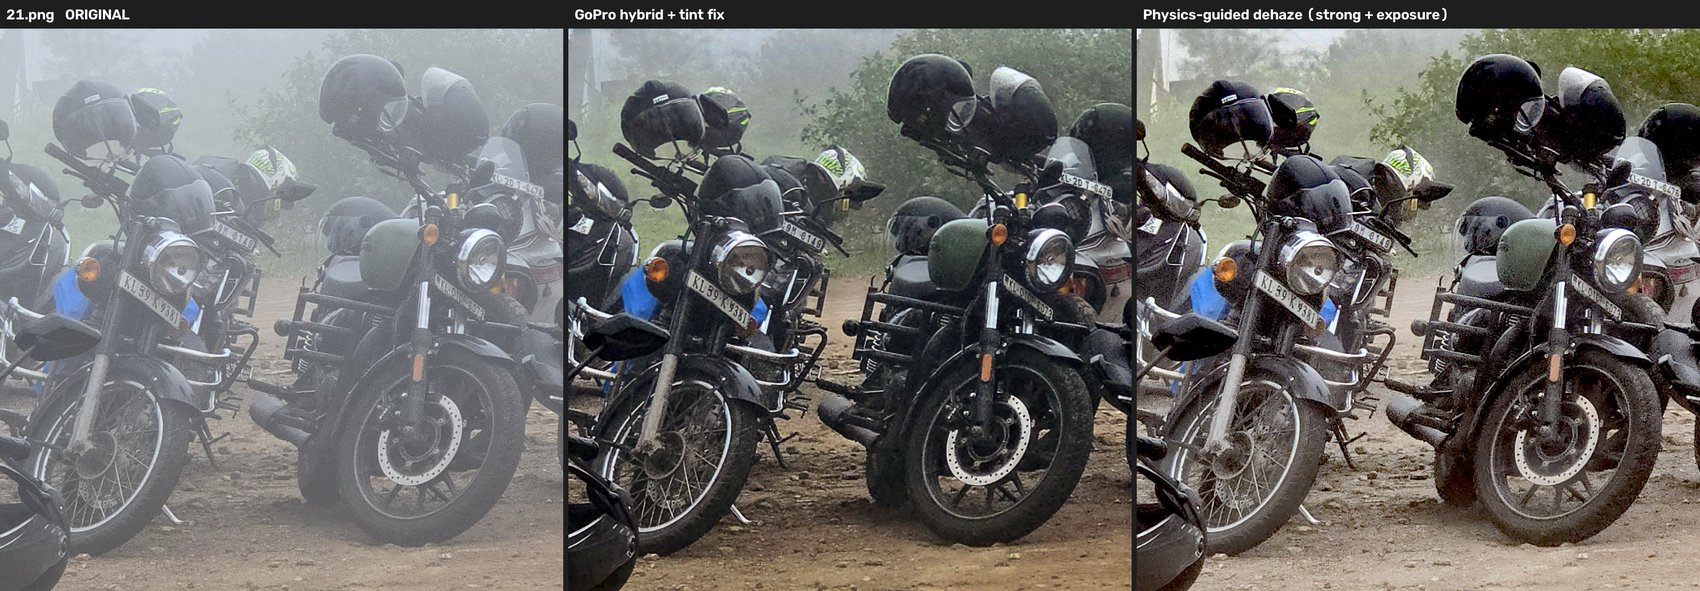
\includegraphics[width=\textwidth]{ponmudi_cmp_bikes.jpg}\\[4pt]
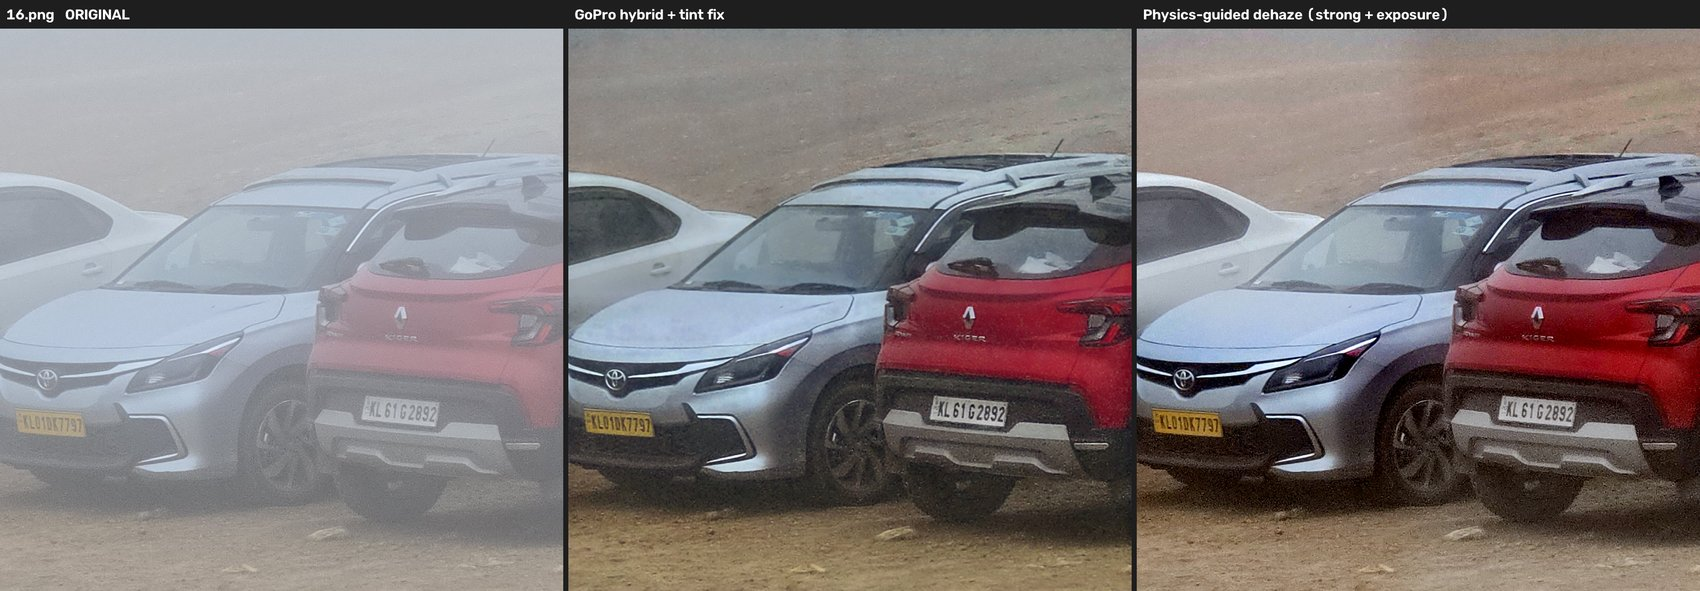
\includegraphics[width=\textwidth]{ponmudi_cmp_suv.jpg}
\caption{Real fog at Ponmudi. In each row: original photograph (left), UVMNet
GoPro-hybrid model with tint fix (middle), physics-guided dehaze, strong with
exposure match (right).}
\label{fig:ponmudicmp}
\end{figure}

\begin{figure}[t]
\centering
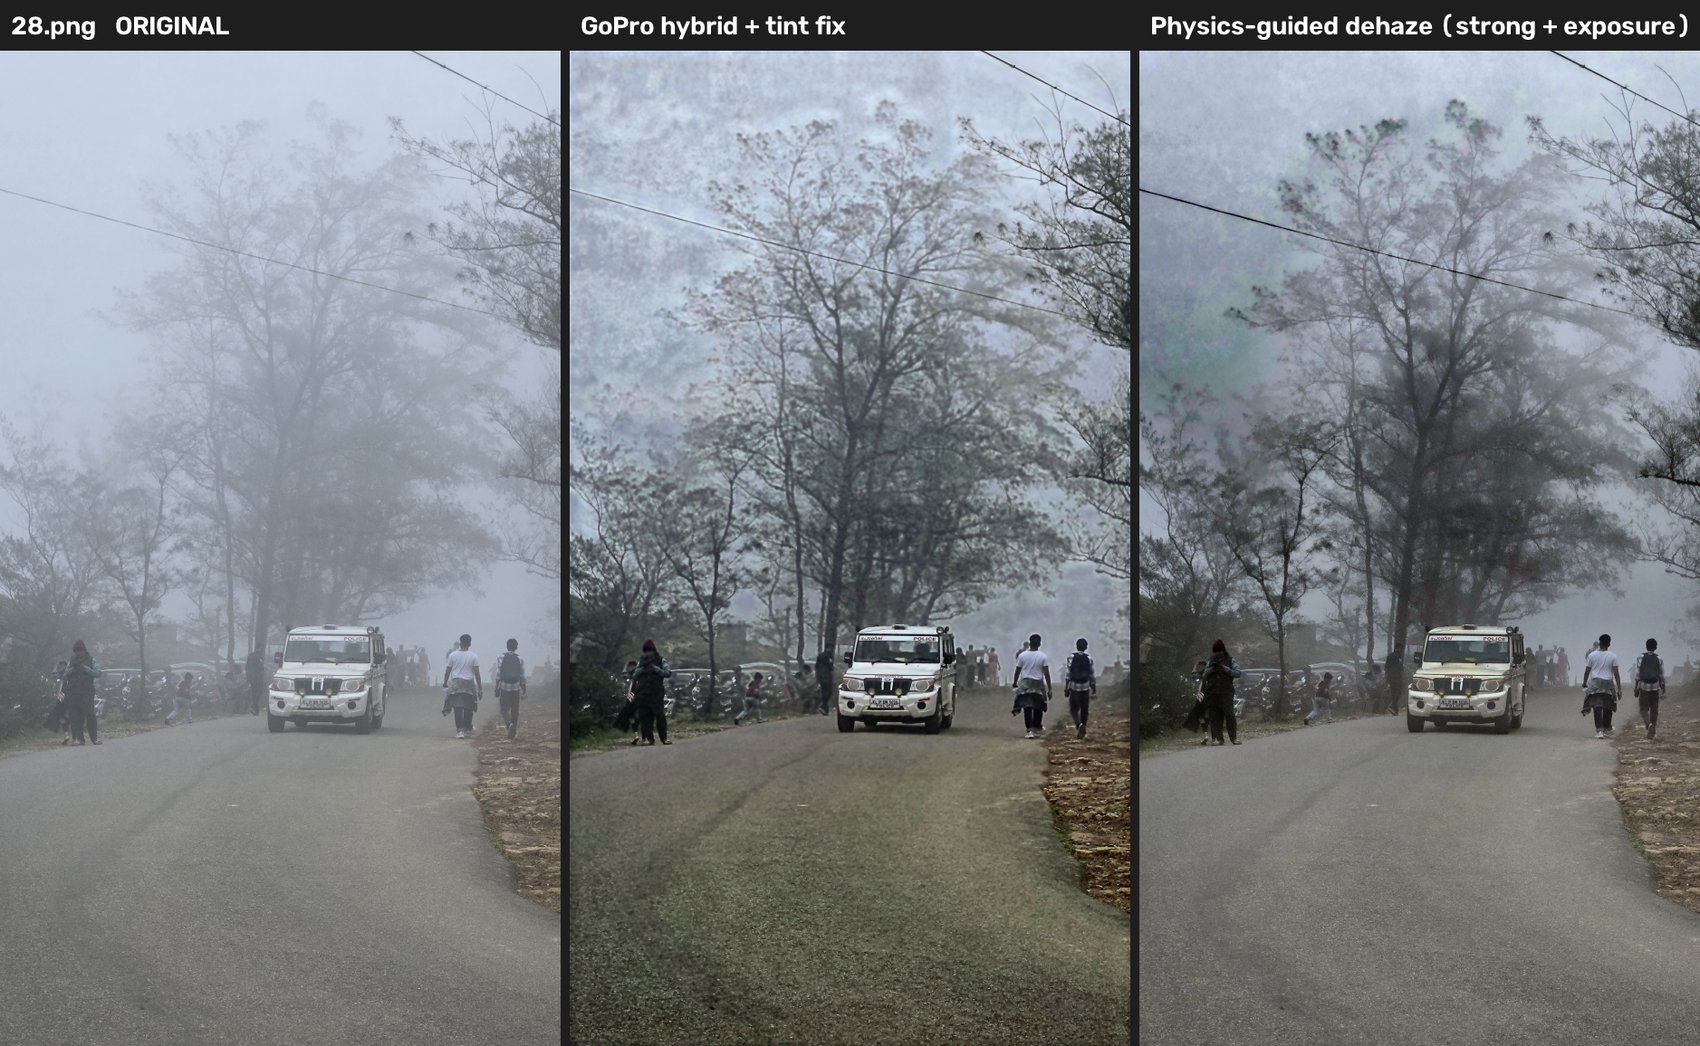
\includegraphics[width=0.55\textwidth]{ponmudi_cmp_road_a.jpg}
\caption{A distant scene on the hill road: original, UVMNet GoPro-hybrid model
with tint fix, physics-guided dehaze.}
\label{fig:ponmudiroad}
\end{figure}

\subsection{Deraining}
\label{sec:derain}

Rain streaks, spray and headlight glare obscure plate characters, so a deraining
module was developed as a second preprocessing stage. Two models were
evaluated.

\paragraph{PW-FNet in stages.} PW-FNet was trained in three stages and evaluated
on a held-out synthetic plate test set and on real rainy plate photographs. On
the synthetic set it raised PSNR from 26.61 to 36.46~dB and SSIM from 0.8918
to 0.9853, and heavily rain-occluded plates were fully recovered
(Figure~\ref{fig:pwfnet}a). To close the synthetic-to-real gap a further
fine-tune on real rain/clean pairs (GT-RAIN) was tried: fine-tuning on real data
alone caused catastrophic forgetting (plate PSNR fell to 20.64~dB), while a mixed
fine-tune preserved plate performance (35.21~dB) but gave only a negligible
real-rain gain (23.64 against 23.60~dB). On independently sourced real rainy
photographs the model partly responded to camera-captured streak rain but left
streaks dimmed rather than removed, and had no measurable effect on road splash
and wet-surface sheen (Figure~\ref{fig:pwfnet}b).

\begin{figure}[t]
\centering
\begin{subfigure}[b]{0.62\textwidth}
  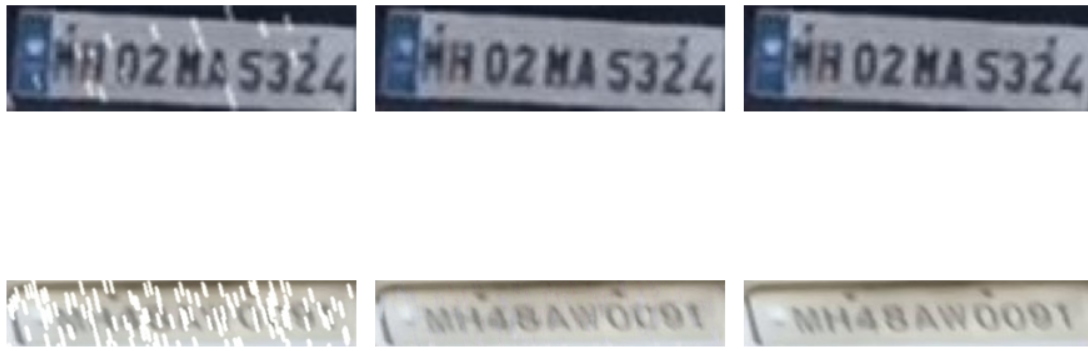
\includegraphics[width=\textwidth]{derain_pwfnet_synthetic.png}
  \caption{Synthetic test plates: rainy, restored, ground truth.}
\end{subfigure}\hfill
\begin{subfigure}[b]{0.33\textwidth}
  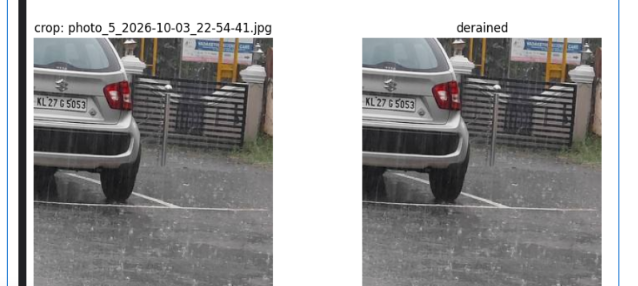
\includegraphics[width=\textwidth]{derain_pwfnet_real.png}
  \caption{Real rain: input and restored.}
\end{subfigure}
\caption{PW-FNet deraining.}
\label{fig:pwfnet}
\end{figure}

\paragraph{A lightweight network for the edge.} A custom U-Net-style network
(named A5) with about 1.72 million parameters was trained from scratch on clean
images from the RodoSol-ALPR dataset~\cite{laroca2022rodosol} paired with
synthetic rain; its architecture is shown in Figure~\ref{fig:a5arch}. The
variants A, A2, A3, A4 and A5 share the architecture and differ in the
synthetic rain generation and fine-tuning; A5 gave the best results on the
synthetic test set. Training used AdamW with an initial learning rate of
$2\times10^{-4}$, a cosine schedule, mixed precision, $256\times256$ crops and a
batch size of four, with the loss
\[
  \mathcal{L} = \mathcal{L}_{\text{Charbonnier}} + 0.2\,\bigl(1-\text{SSIM}\bigr),
\]
and an extra weight on the plate region so that plate detail is preserved. The
pretrained NeRD-Rain~\cite{chen2024nerdrain} was kept as a comparison baseline.

\begin{figure}[t]
\centering
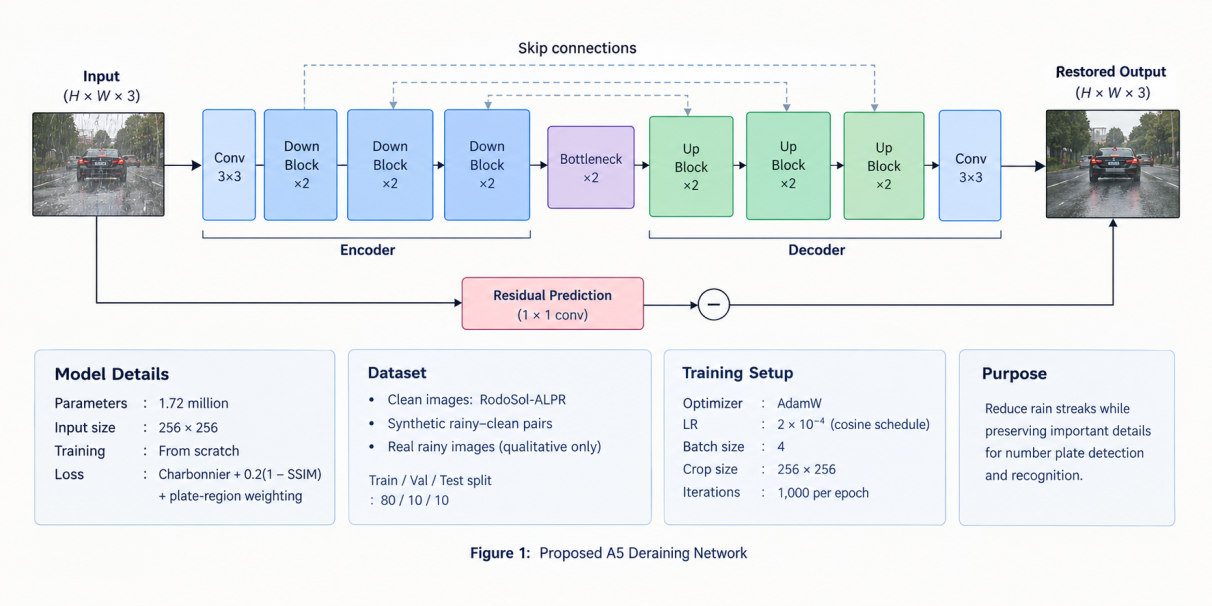
\includegraphics[width=0.9\textwidth]{derain_a5_architecture.png}
\caption{Architecture of the lightweight A5 deraining network.}
\label{fig:a5arch}
\end{figure}

On a 30-image synthetic test set A5 reached 29.19~dB, 7.02~dB above the
unprocessed input and clearly above NeRD-Rain and the earlier variant A4
(Table~\ref{tab:rain}). On real rainy-road photographs and video frames there is
no clean reference, so the evaluation is visual: some streaks are reduced
(Figures~\ref{fig:a5real} and~\ref{fig:a5cmp}), but dense rain, headlight glare and
road spray remain. Neither deraining model has yet been shown to raise plate
reading on real rain, so deraining is carried to Phase~2 as an open item.

\begin{table}[t]
\centering
\caption{Deraining on the 30-image synthetic test set (PSNR in dB).}
\label{tab:rain}
\small
\begin{tabular}{@{}lccc@{}}
\toprule
\textbf{Method} & \textbf{PSNR} & \textbf{Tone-matched PSNR} & \textbf{Plate-region PSNR}\\
\midrule
No deraining & 22.17 & 26.90 & 22.11\\
NeRD-Rain (pretrained) & 20.98 & 26.35 & 19.61\\
A4 & 25.61 & 26.31 & 25.76\\
A5 & \textbf{29.19} & \textbf{29.82} & \textbf{26.99}\\
\bottomrule
\end{tabular}
\end{table}

\begin{figure}[t]
\centering
\begin{subfigure}[b]{0.48\textwidth}
  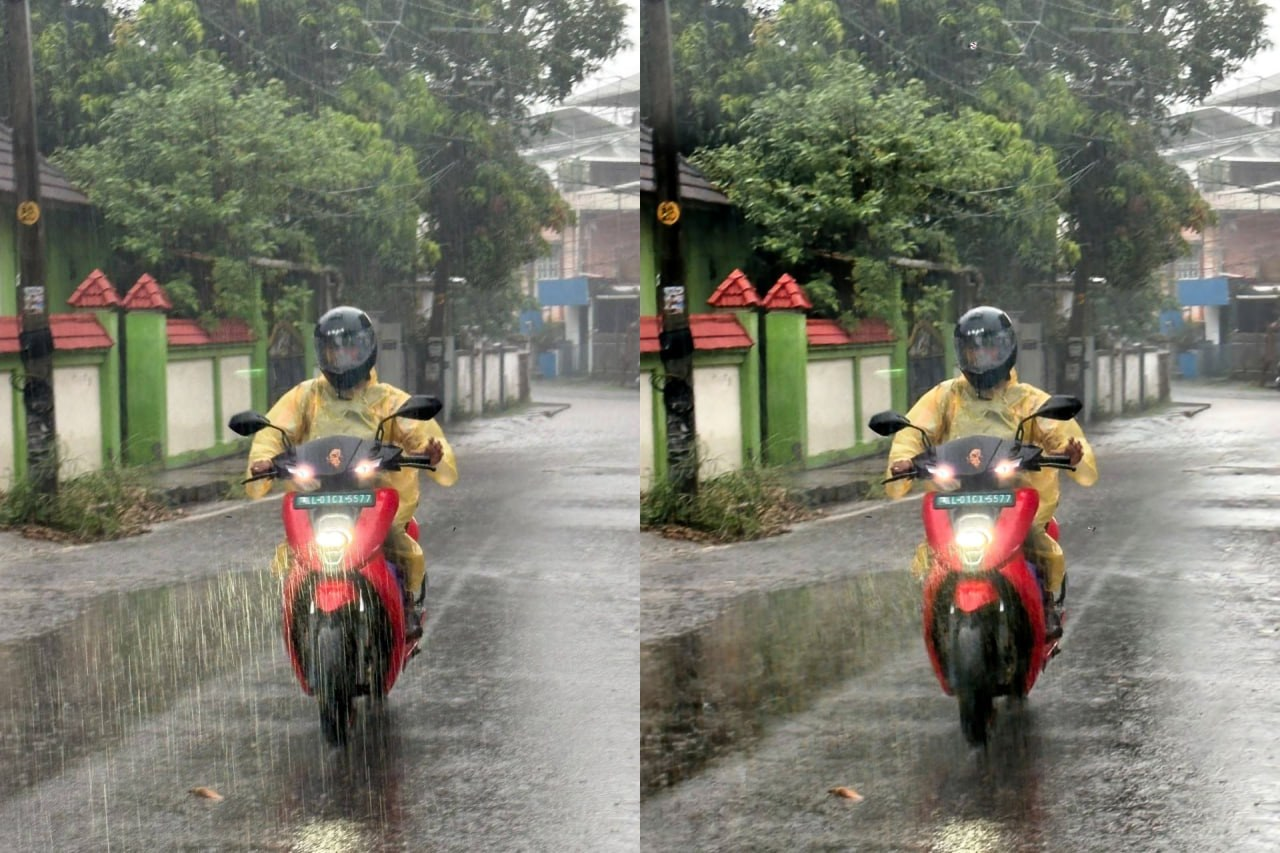
\includegraphics[width=\textwidth]{derain_a5_motorcycle.jpg}
  \caption{Motorcycle scene.}
\end{subfigure}\hfill
\begin{subfigure}[b]{0.48\textwidth}
  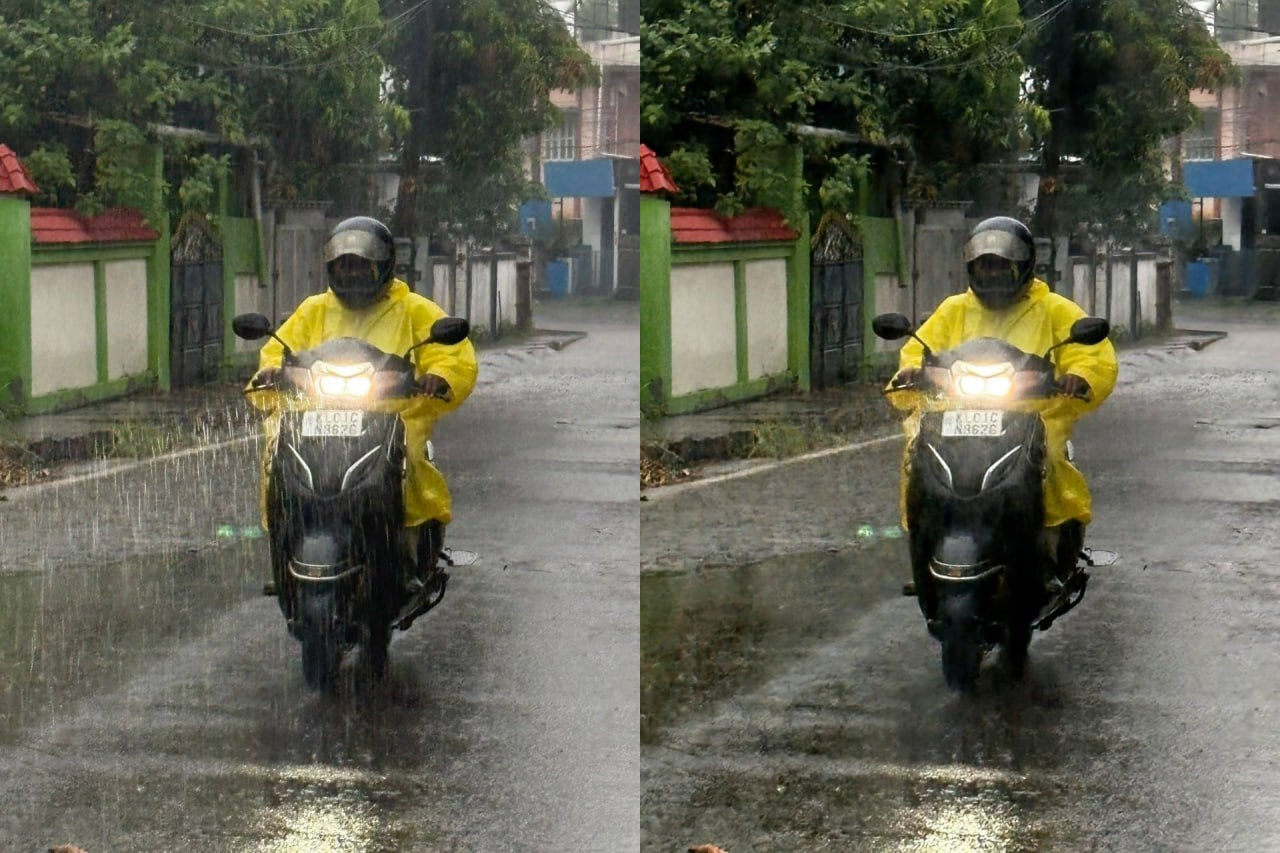
\includegraphics[width=\textwidth]{derain_a5_scooter.jpg}
  \caption{Scooter scene.}
\end{subfigure}
\caption{Real rain: original (left) and A5-restored output (right).}
\label{fig:a5real}
\end{figure}

\begin{figure}[t]
\centering
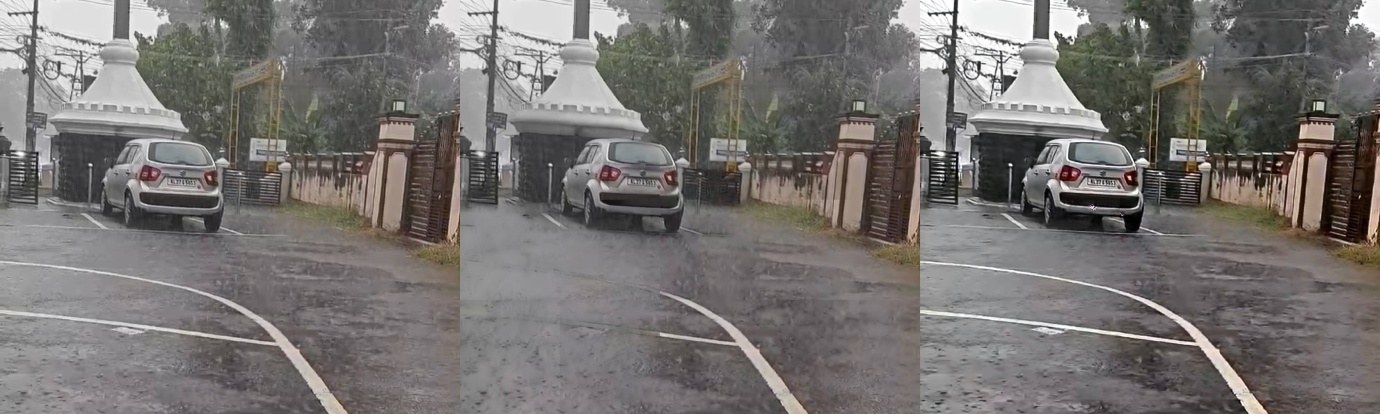
\includegraphics[width=0.9\textwidth]{derain_compare_nerd_a5.jpg}
\caption{Same input image: original, NeRD-Rain and A5 outputs.}
\label{fig:a5cmp}
\end{figure}

\subsection{Discussion}

Restoration helps the \emph{viewer} more than the \emph{reader}. On synthetic
data every learned model improves PSNR, and for fog the physics-guided pictures
are clearly cleaner, but the plates read on real photographs rise only a few
percent and always within the noise of the test. Two practical rules follow:
choose the restoration route by weather and by the purpose (display or
recognition), and put the effort into a reader that is robust to degraded
plates and into combining frames, which are described next.

% ---------------------------------------------------------------------
\section{Plate Recognition}
\label{sec:lprnet}

\subsection{OCR baselines}

\paragraph{EasyOCR.} With $3\times$ upscaling, histogram equalisation and an
alphanumeric allow-list the output was mostly garbled: confidence was 0.06--0.46
on the first test image and 0.11--0.61 across ten test images, and the plate
\plate{KL01BM5673} came back as strings such as \plate{KLYGIBH5673}. On 218
hand-labelled scenes the exact-match rate was only 17--25\,\% in fog (light fog
25\,\%, severe fog 17\,\%) and 6--11\,\% in rain, with a character error rate of
0.45--0.74 (Figure~\ref{fig:easyocr}). EasyOCR is a general scene-text reader; it
confused \plate{1}/\plate{I} and \plate{7}/\plate{Z} and failed on small
blurred plates.

\paragraph{Other readers.} PaddleOCR could not be run to completion (an internal
inference-engine error of its Windows CPU build). The plate-specific
\emph{fastplateOCR} was clearly better and read \plate{KL01BM5673} as
\plate{KL01BM567}, 9 of 10 characters correct, but it consistently dropped
the trailing digit of 10-character Indian plates and its repeated readings of
one plate varied (Figure~\ref{fig:ocr}). This was the decision point to build a
reader for Indian plates.

\begin{figure}[t]
\centering
\begin{subfigure}[b]{0.56\textwidth}
  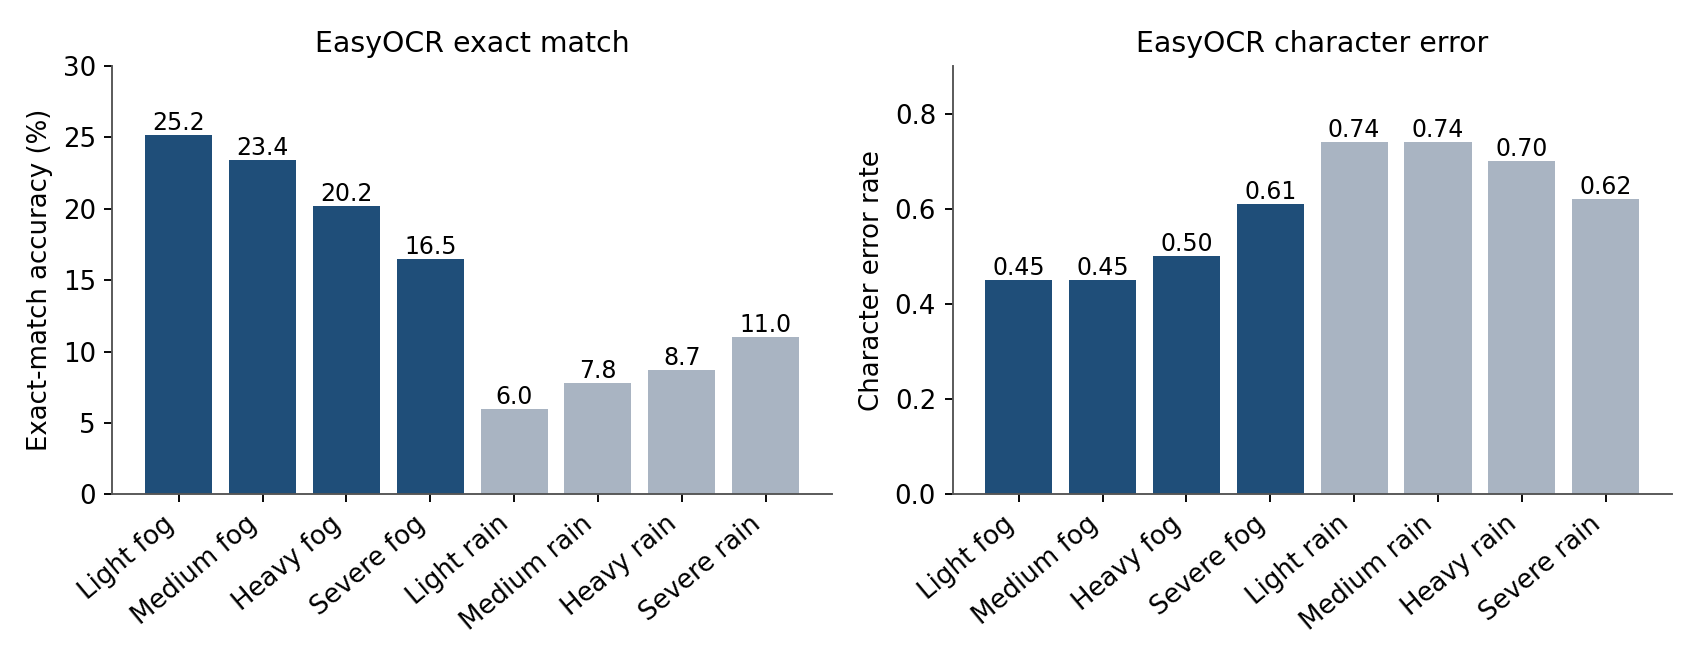
\includegraphics[width=\textwidth]{easyocr_weather.png}
  \caption{EasyOCR exact match and character error by weather.}
  \label{fig:easyocr}
\end{subfigure}\hfill
\begin{subfigure}[b]{0.40\textwidth}
  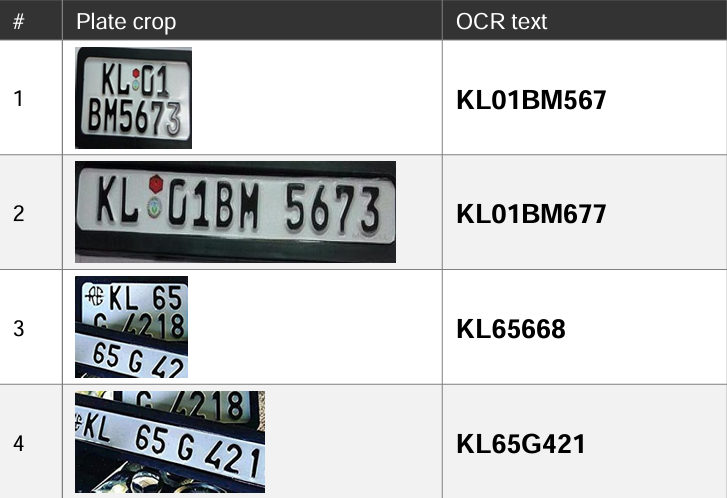
\includegraphics[width=\textwidth]{ocr_baselines.png}
  \caption{Readings of the baseline OCR engines on sample plates.}
  \label{fig:ocr}
\end{subfigure}
\caption{Baseline OCR results.}
\end{figure}

\subsection{LPRNet}

LPRNet~\cite{zherzdev2018lprnet} is a convolutional network that reads the whole
plate in one pass. The plate crop is resized to $200\times24$ pixels and the
network outputs, for each of its horizontal positions, a probability over the 36
characters A--Z and 0--9 and a CTC blank. With the CTC loss~\cite{graves2006ctc}
the training target is the plate string and no per-character boxes are needed.
Two-line plates (common on two-wheelers, autos and some cars) are flattened
into one row before reading by cutting the crop at its horizontal midline and
placing the lower half after the upper one. For crops whose aspect ratio is
ambiguous (between 1.9 and 2.6) both readings, single-line and flattened, are
made and the plate-looking, higher-confidence one is kept.

\subsection{Training in stages}

Trained from scratch on the 218 labelled scenes the network overfitted
badly: the training loss fell to 0.32 but the validation exact match stayed at
0--6\,\% with a character error rate of 0.70, because the data held only about
197 distinct plates. Pre-training on synthetic plates (30\,000 random plates per
epoch) raised the synthetic validation accuracy from 78.5\,\% to 99.5\,\%,
showing that the network was sound and that diversity of data was the limit.
Each later step added a kind of data that the earlier readers lacked
(Table~\ref{tab:lpr}):
\begin{itemize}
  \item \textbf{Fine-tuning and mixing.} Fine-tuning on the real plates gave
        34--37\,\% exact match with a character error of 0.32; mixing synthetic
        plates into the fine-tuning and adding 40\,000 images of the CCPD
        set~\cite{xu2018ccpd} lowered the character error to 0.249 (44\,\%
        exact; Figure~\ref{fig:lprcer}).
  \item \textbf{Real Indian plates.} The reader was fine-tuned on normal and
        CAPTCHA-style crops after removing about 10\,\% junk, on our own Kerala
        photographs labelled with a review page, and on the public Zenodo
        plate set (about 1\,355 pairs). With 16 Kerala plates held out as a fixed
        test, exact reads rose from a mean of 6.7 to 9.0 of 16 over three seeds.
        Because every retrain broke different plates, results are reported over
        multiple seeds and the weights of the best runs are averaged.
  \item \textbf{Degradation.} Training with shrinking to 12--30 pixels height,
        blur, motion and JPEG compression halved the character error on small
        video plates (0.50 to about 0.31).
  \item \textbf{Repeated characters.} CTC drops one of repeated characters
        (\plate{KL21AA2696} read with one \plate{A}, \plate{888} read as
        \plate{88}); synthetic plates with repeated characters raised per-frame
        exact reads on a video from 14\,\% to about 46\,\%.
  \item \textbf{Real video crops.} A review page (\code{video\_label\_review})
        turns each tracked plate in traffic videos into labelled crops from one
        typed label. Round~1 (114 plates, 4\,926 crops) raised exact plates on
        an unseen video from 19 to 22 of 27; round~2 (93 more plates, 1\,850
        crops) raised six held-out test videos from 38 to 41 of 51 plates
        (Figure~\ref{fig:realgain}). The test videos were never used for
        training.
  \item \textbf{Hard cases.} Photographs of 250 Rajasthan plates showed that
        Delhi plates with a lettered RTO code (\plate{DL3CCU5010}) had no
        layout, that \plate{Q} made up only 0.37\,\% of real characters
        and that red temporary plates had never been seen; a layout was added
        and synthetic plates with red backgrounds and \plate{Q} were generated.
        Exact reads on 62 held-out crops rose from 48 to 56, with the video
        benchmark unchanged (75 against 74--75).
\end{itemize}

\begin{table}[t]
\centering
\caption{Progress of the plate reader. CER is the character error rate.}
\label{tab:lpr}
\small
\begin{tabularx}{\textwidth}{@{}Xp{4.6cm}@{}}
\toprule
\textbf{Step} & \textbf{Result}\\
\midrule
Trained from scratch on 218 scenes & 0--6\,\% exact, CER 0.70\\
Synthetic pre-training + real fine-tune & 34--37\,\% exact, CER 0.32\\
+ CCPD and synthetic mixing & 44\,\% exact, CER 0.249\\
+ Zenodo plates (Kerala, 16 held out) & 6.7 to 9.0 of 16 exact\\
+ degradation training (small video plates) & CER 0.50 to 0.31\\
+ repeated-character synthetic plates & per-frame exact 14\,\% to 46\,\% (video)\\
+ real video crops, rounds 1 and 2 & 19 to 22 of 27; 38 to 41 of 51\\
+ Rajasthan plates, red plates, \plate{Q} & 48 to 56 of 62 (held-out crops)\\
\bottomrule
\end{tabularx}
\end{table}

\begin{figure}[t]
\centering
\begin{subfigure}[b]{0.62\textwidth}
  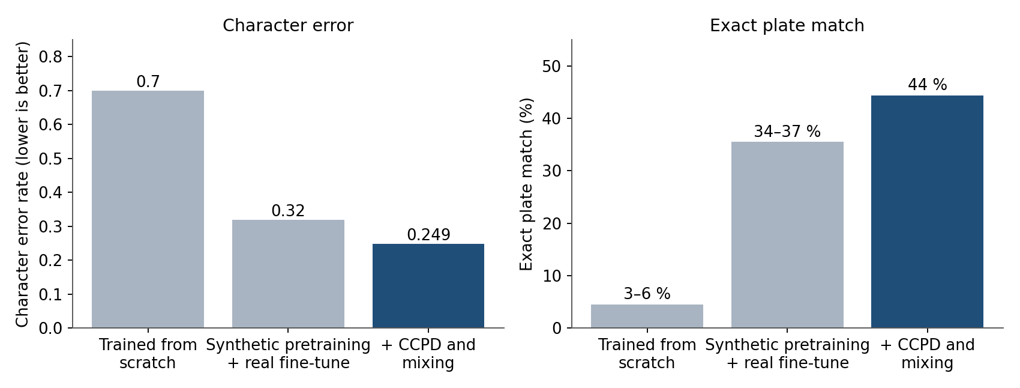
\includegraphics[width=\textwidth]{lprnet_cer_exact.png}
  \caption{Character error and exact match.}
  \label{fig:lprcer}
\end{subfigure}\hfill
\begin{subfigure}[b]{0.34\textwidth}
  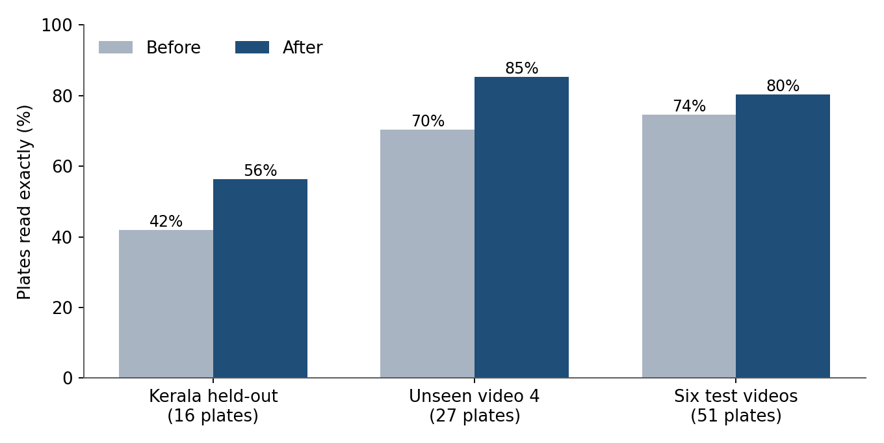
\includegraphics[width=\textwidth]{real_data_gain.png}
  \caption{Plates read before and after real-data training.}
  \label{fig:realgain}
\end{subfigure}
\caption{LPRNet results.}
\label{fig:lprresults}
\end{figure}

\subsection{Format-constrained decoding}

The raw CTC output is corrected with the structure of Indian plates. A plate is
two letters (state), two digits (district), one or two letters (series) and
four digits, \eg\ \plate{KL01AB1234}; layouts for 9-character and 10-character
plates, for the 9-character Delhi style and for Delhi plates with a lettered
RTO code are known to the decoder. Instead of replacing letters and digits
with a fixed table (\plate{O}$\rightarrow$\plate{0}), the decoder uses the
network's own per-position probabilities, restricted to the characters that the
layout allows at each slot, so that characters such as \plate{Q} that a fixed
swap would destroy are recovered. Detections that do not look like a plate
(road signs, bag logos) are hidden by default.

\subsection{Reading weather-degraded plates}

A reader trained for weather (with fog and haze applied to the training crops)
and a ``select'' view that chooses between the plain and the smoothed crop gave
the best reading of the Ponmudi photographs (47--51 of 85, against 40 for the
installed reader untouched; Section~\ref{sec:ponmudi}). The installed default
reader is the result of the real-video and Rajasthan rounds above; the
weather-trained readers are kept as separate checkpoints and are evaluated
before any replacement.

% ---------------------------------------------------------------------
\section{Tracking and Real-Time Operation}
\label{sec:realtime}

\subsection{Reading plates from video}

A first video reader detected plates in every frame, tracked each plate, read
it repeatedly and took a vote over the readings, preferring readings that match
the strict plate format. A track is called reliable when at least five reads
agree and they make up at least 4\,\% of its reads. The medoid of the readings
(the reading closest to all others) is used when no clear majority exists.

\subsection{Real-time pipeline}

The offline reader took about 10 minutes for a 45~s, 1080p clip, which is not
usable for a system that must show a plate as the vehicle passes. Profiling
showed that recognition took 30\,\% of the time, detection 27\,\%, video writing
18\,\% and the per-frame vote 15\,\% (and growing with track length). The
real-time version updates the vote incrementally over the most frequent
readings, reads each plate on every frame at first (the first ten reads) and
then every third frame, stops reading a plate once its vote is stable, runs the
detector in half precision, and skips frames when it falls behind. It processed
the 45~s clip in 44~s, about 55 frames per second at 1080p, with accuracy equal
to the offline reader (20 of 27 plates on the benchmark video;
Figure~\ref{fig:speed}). Plates that stay in view for only a few frames are
announced when they leave, if the reading is well formed (at least three agreeing
reads and 30\,\% agreement).

Reading and detection run in parallel worker processes, each with its own
detector and reader, with frames passed through shared memory and results
re-ordered into frame order; tracking and voting stay in one place so that the
output is identical to the single-process run. On 4K footage the ceiling is the
CPU decoding rate of about 27 frames per second (Table~\ref{tab:fps}).

\begin{table}[t]
\centering
\caption{Throughput in frames per second for different numbers of worker
processes (no frame skipping).}
\label{tab:fps}
\small
\begin{tabular}{@{}lcccc@{}}
\toprule
\textbf{Video} & \textbf{1 process} & \textbf{2 workers} & \textbf{4 workers} & \textbf{6 workers}\\
\midrule
1080p, 60 fps & 40.9 & 51.5 & 61.8 & 47.0\\
4K & 13.5 & 19.7 & 19.0 & 16.5\\
\bottomrule
\end{tabular}
\end{table}

\begin{figure}[t]
\centering
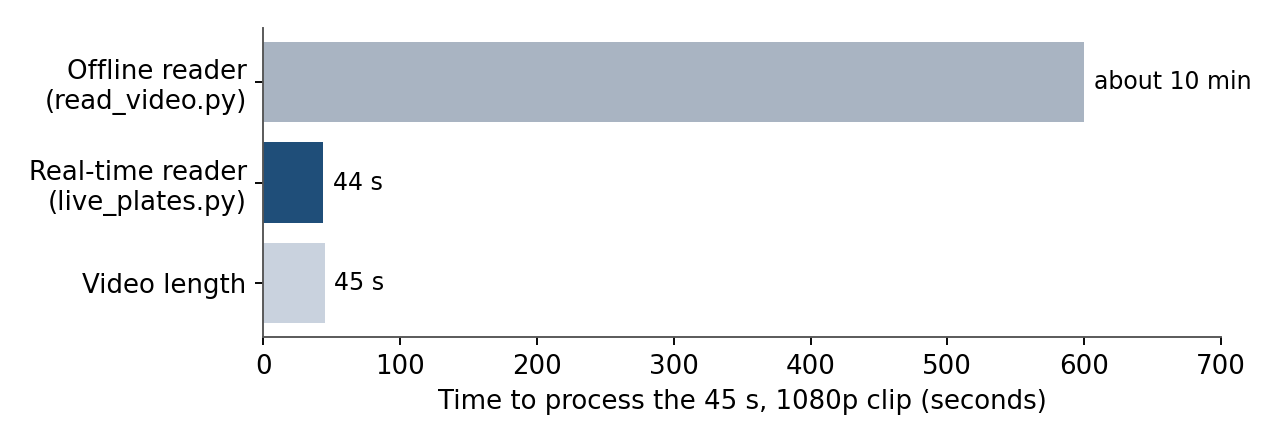
\includegraphics[width=0.75\textwidth]{offline_vs_live_time.png}
\caption{Time to process a 45~s, 1080p clip with the offline reader and the
real-time pipeline.}
\label{fig:speed}
\end{figure}

% ---------------------------------------------------------------------
\section{Tests on Unseen Traffic Videos}
\label{sec:video}

\paragraph{First test video (1.MOV, 4K).} Thirteen plates were announced. Ten of
the twelve real plates were read exactly (Table~\ref{tab:vid1}). One plate lost a
digit (\plate{KL2C6050} for \plate{KL20C6050}), one plate partly hidden by a
shadow could not be verified, and a phone-number sign on a scooter was
announced as a plate (\plate{BP20OB9200}). One yellow-plate vehicle was not
announced because the readings of its bottom-line letter split between several
characters. The live view and the announced plates are shown in
Figures~\ref{fig:live} and~\ref{fig:announced}.

\begin{figure}[t]
\centering
\begin{subfigure}[b]{0.48\textwidth}
  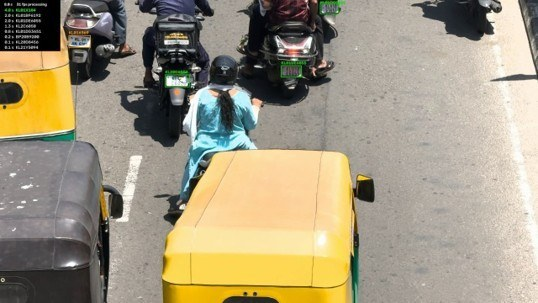
\includegraphics[width=\textwidth]{live_view_1.jpg}
\end{subfigure}\hfill
\begin{subfigure}[b]{0.48\textwidth}
  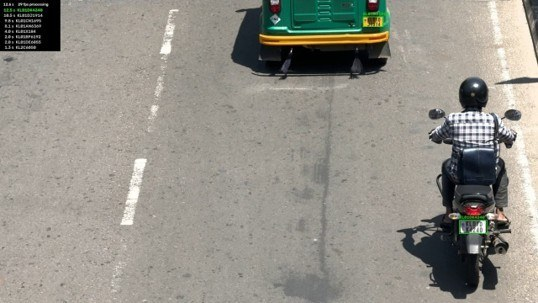
\includegraphics[width=\textwidth]{live_view_2.jpg}
\end{subfigure}
\caption{Live output: plate boxes with readings, and the list of confirmed
plates with their times at the top left; the second frame is a few seconds later.}
\label{fig:live}
\end{figure}

\begin{figure}[t]
\centering
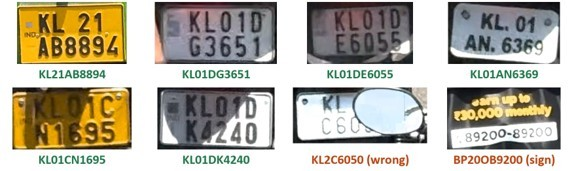
\includegraphics[width=0.8\textwidth]{announced_plates.png}
\caption{Plate crops and the readings announced: six correct, one dropped digit,
one sign read as a plate.}
\label{fig:announced}
\end{figure}

\begin{table}[t]
\centering
\caption{Results on the first test video.}
\label{tab:vid1}
\small
\begin{tabularx}{\textwidth}{@{}llX@{}}
\toprule
\textbf{Outcome} & \textbf{Plates} & \textbf{Detail}\\
\midrule
Read exactly & 10 of 12 & \plate{KL21AB8894}, \plate{KL21Y5094}, \plate{KL20D8456}, \plate{KL01DG3651}, \plate{KL01DE6055}, \plate{KL01BF6192}, \plate{KL01AN6369}, \plate{KL01CN1695}, \plate{KL01DJ1914}, \plate{KL01DK4240}\\
Wrong & 1 & \plate{KL2C6050} (true \plate{KL20C6050})\\
Not verifiable & 1 & \plate{KL01X184} (plate partly hidden by a shadow)\\
Not a plate & 1 announcement & \plate{BP20OB9200} (phone-number sign)\\
Not announced & 1 vehicle & yellow plate \plate{KL01C?7591}, bottom-line letter unclear\\
\bottomrule
\end{tabularx}
\end{table}

\paragraph{Other unseen footage.} On a 4K video from a second set (video 7) the
reader confirmed 40 plates; checked by eye, about 31 were right, 6 wrong and 3
uncertain, and about 3 real vehicles were never confirmed because their plates
were blurred or faded. Reading every frame for a plate's first ten reads and
announcing short passes on exit were added after this test to catch fast
vehicles. After the later real-video rounds the benchmark video gave 23 of 27
plates exactly.

\paragraph{Known failures.} Three equal digits in a row are still dropped
(\plate{KL01CH4448} read as \plate{KL01CH448}), series from other states are weaker,
and blurred or faded plates and signs cause misses or false plates. Plates only
22--39 pixels wide on two-wheelers and autos remain unreadable; footage of
higher resolution is the main remaining lever for them.

% ---------------------------------------------------------------------
\section{Foggy Video Pipeline}
\label{sec:foggyvideo}

The pieces of this chapter were combined into a single pipeline for foggy
video: UVMNet (GoPro-trained) followed by the physics-guided dehaze (strong,
$\gamma=1.25$, with the veil colour and exposure smoothed over time),
then the YOLOv11 detector (1280 pixels, confidence 0.25) and finally the
installed LPRNet with the ``select'' view and format correction. It was run on
four short clips filmed in fog at Ponmudi (133, 161, 144 and 237 frames at
about 29 frames per second).

Two features make the result easy to inspect. First, the annotated video
\emph{slows down} by a factor of four while a plate is detected (and for four
frames afterwards), so that the annotation can be followed. Second, a box at
the top left shows, for up to three vehicles, an enlarged crop of the plate in
the current frame, the \emph{final} reading and its votes. The final reading is
the most voted reading of that vehicle over the whole clip and is fixed from the
first frame in which the vehicle appears, so that the number does not change
from frame to frame. Raw tracks that are interrupted for at most 15 frames and
whose boxes are close are merged into one vehicle before the vote.
Figure~\ref{fig:foggyvid} shows frames of the output.

\begin{figure}[t]
\centering
\begin{subfigure}[b]{0.48\textwidth}
  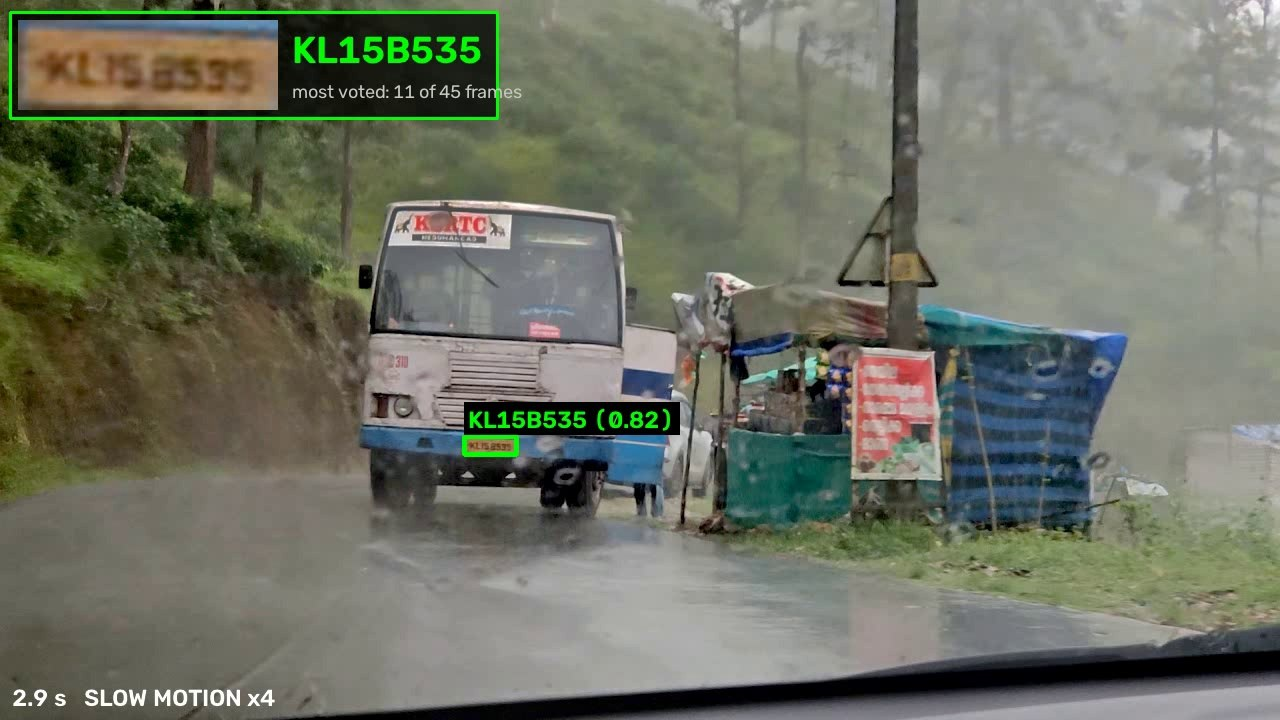
\includegraphics[width=\textwidth]{foggy_video_bus.jpg}
  \caption{A bus on the hill road.}
\end{subfigure}\hfill
\begin{subfigure}[b]{0.48\textwidth}
  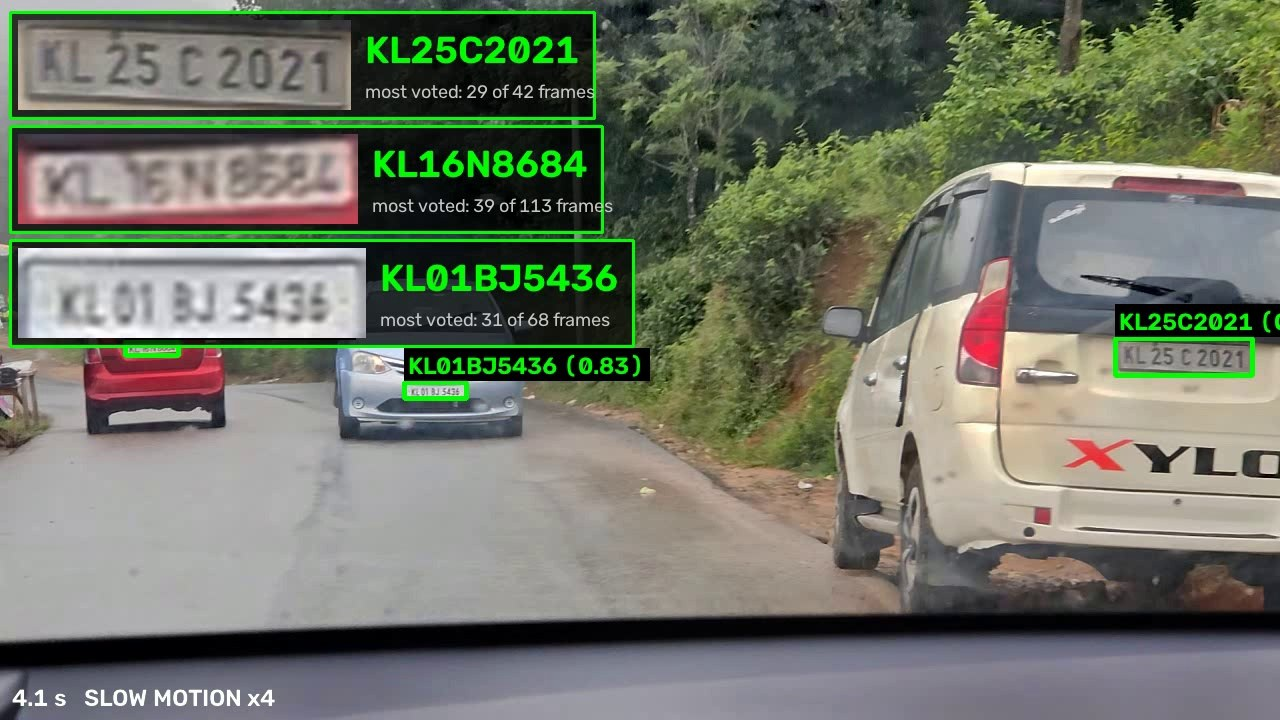
\includegraphics[width=\textwidth]{foggy_video_multi.jpg}
  \caption{Three vehicles tracked at once, each with its final reading.}
\end{subfigure}
\caption{Frames of the annotated foggy video output (slow motion $\times4$).}
\label{fig:foggyvid}
\end{figure}

\begin{figure}[t]
\centering
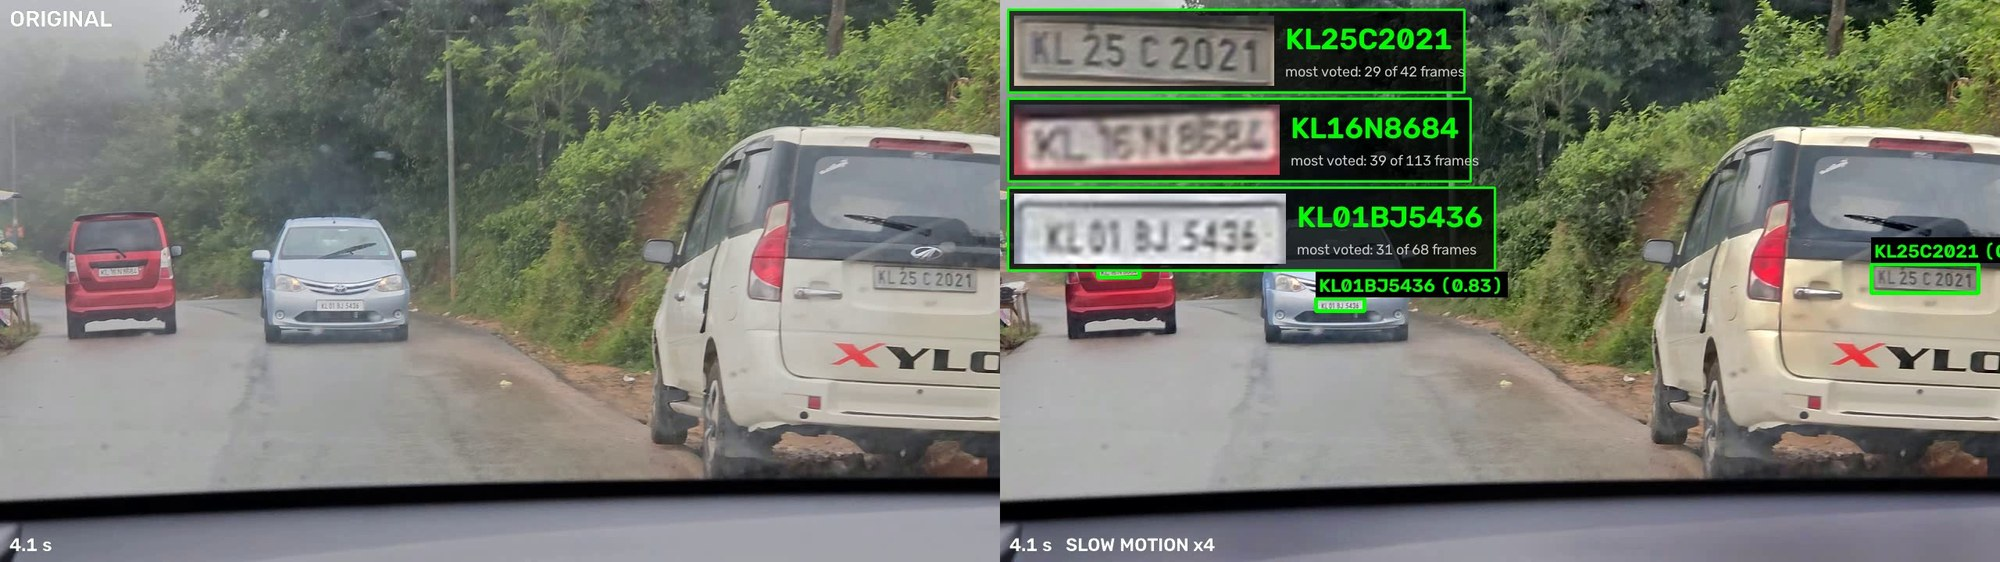
\includegraphics[width=\textwidth]{foggy_video_side.jpg}
\caption{Original (left) and dehazed, annotated (right) frame of the same
clip.}
\label{fig:foggyside}
\end{figure}

Table~\ref{tab:foggyvehicles} lists the vehicles found. The vote share is the
fraction of the vehicle's readings that agree with the final number, and is a
measure of how much to trust it. The numbers are the output of the system; the
plate crops of \plate{KL25C2021}, \plate{KL16N8684} and \plate{KL01BJ5436} agree
with the final readings by eye, whereas the readings with a vote share below
about 35\,\% (video~1, video~3) should be regarded as unconfirmed. A complete
ground-truth check of these four clips has not been done.

\begin{table}[t]
\centering
\caption{Vehicles found in the four foggy clips (final reading = most voted).}
\label{tab:foggyvehicles}
\small
\begin{tabular}{@{}llccc@{}}
\toprule
\textbf{Video} & \textbf{Final reading} & \textbf{Frames seen} & \textbf{Votes} & \textbf{Share}\\
\midrule
1  & \plate{TN10BJ0282} & 20 & 3 & 15\,\%\\
2  & \plate{KL22Q7925}  & 20 & 11 & 55\,\%\\
3  & \plate{KL15B535}   & 45 & 11 & 24\,\%\\
b1 & \plate{KL01CH7254} & 48 & 30 & 62\,\%\\
b1 & \plate{KL25C2021}  & 42 & 29 & 69\,\%\\
b1 & \plate{KL16N8684}  & 113 & 39 & 35\,\%\\
b1 & \plate{KL01BJ5436} & 68 & 31 & 46\,\%\\
b1 & \plate{KL364848}   & 2 & 1 & 50\,\%\ (unreliable)\\
\bottomrule
\end{tabular}
\end{table}

\subsection{Combining frames of the same plate}
\label{sec:fusion}

Single photographs are limited by information, but a video holds many views of
a plate. For each tracked plate up to 16 sharp crops are aligned to the
sharpest one with an affine ECC registration~\cite{evangelidis2008ecc},
upsampled by two, and combined by a weighted mean or a median; the combined
image is then read. The Ponmudi videos gave 133 plate tracks, of which nine
could be matched to verified plates, read by four readers (36 readings). A
single, widest frame gave 1 of 36 exactly right, a vote over the frames of the
track 9, and the fused image 8 (weighted mean) to 10 (median)
(Figure~\ref{fig:fusion}). The fused images are far cleaner than any single
frame, but on this small set fusion is no better than voting; for the plate
\plate{KL10BB8545} the fused image was exactly right for all six tracks
against four for the vote and one for the single frame. Combining
the frames of a vehicle, by vote or by fusion, is the clearest lever for foggy
video.

\begin{figure}[t]
\centering
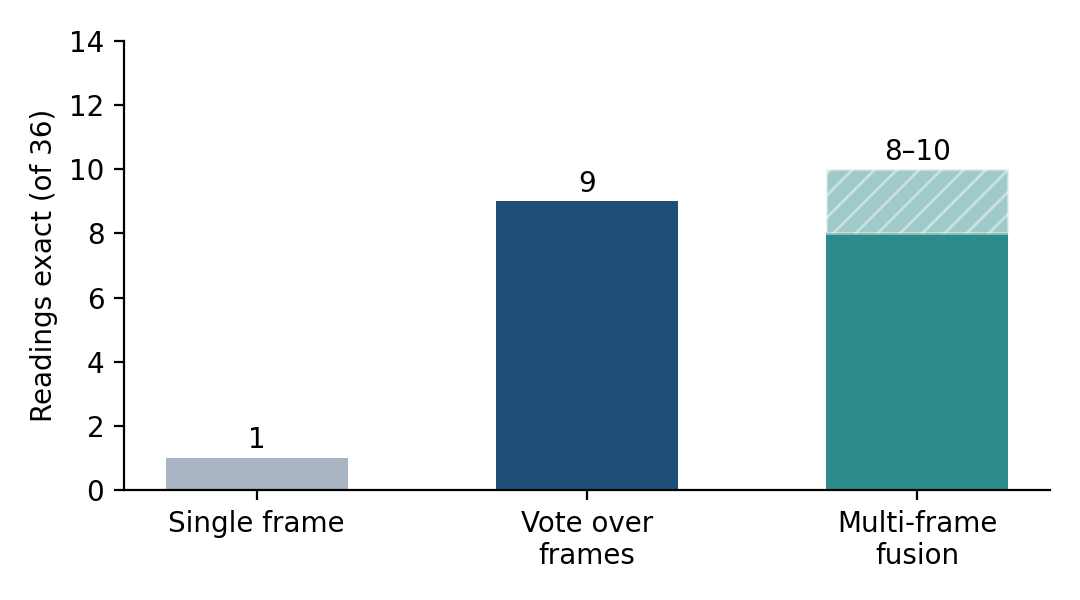
\includegraphics[width=0.6\textwidth]{video_fusion.png}
\caption{Readings exactly right (of 36) from a single frame, a vote over frames
and multi-frame fusion on the Ponmudi tracks (fusion: 8 for the mean, 10 for the
median; the hatched part shows the range).}
\label{fig:fusion}
\end{figure}

% ---------------------------------------------------------------------
\section{Browser Interface}

A browser interface (\code{plate\_app.py}) was written so that the pipeline
can be used without the command line. It lets the user pick or drop videos and
photographs (or type a path), shows the live annotated view with a list of the
confirmed plates, keeps earlier runs, and offers stop, play-back of the
annotated video and a CSV download; the number of parallel workers can be set
on the page. A second version for foggy video (\code{foggy\_plate\_app.py})
runs the UVMNet and physics-guided stages before detection and reading. Both
were tested end to end on videos by path, 4K input and photographs.

% ---------------------------------------------------------------------
\section{Summary}

Phase~1 produced a plate detector with 99.2\,\% mAP@50, a plate reader whose
exact-plate rate was raised in stages with synthetic, public and
self-labelled data, a real-time pipeline that confirms plates by voting at up
to 55 frames per second on 1080p, and fog and rain restoration models with a
physics-guided option for display. The experiments showed that the plate reader
and the combination of frames, rather than ever heavier restoration, decide how
many plates are read in bad weather.

